\documentclass{article}
\usepackage[utf8]{inputenc}
\usepackage{tikz}
\usepackage{pgfplots}
\usepackage{graphicx}
\usepackage{latexsym}
\usepackage{amsmath}

\title{Fondamenti di Telecomunicazioni}
\author{Matteo Zanella}
\date{A.A 2022-2023}

\pgfplotsset{compat=1.18} 
\begin{document}
	
	\maketitle
	
	\section{Segnali}
	
	Un segnale è una funzione del tempo $s(t)\in\Re$, ad esempio una trasmissione su canale analogico/continuo avviene per mezzo di segnali.
	Il tempo può essere considerato come continuo o discreto:\\
	\begin{enumerate}
		\item I segnali a \textbf{tempo continuo} vengono indicati con $y(t)$
		\item I segnali a \textbf{tempo discreto} vengono indicati con $s(KT)$ con $T$ \textbf{quanto temporale}(tempo che intercorre tra due osservazioni sequenziali)
	\end{enumerate}
	I valori assunti dai segnali possono essere:
	\begin{enumerate}
		\item \textbf{continui}: il segnale assume valori $\in\Re$ (o sottoinsiemi)
		\item \textbf{discreti}: il segnale assume valori discreti\\
	\end{enumerate}
	I segnali analogici sono segnali continui con valori continui, mentre i segnali digitali sono segnali discreti con valori discreti.
	
	\subsection{Esempi di segnali}
	
	$$rect(t)=
	\left\{
	\begin{array}{rcrcrcr}
		0&t<\frac{1}{2}\lor t>\frac{1}{2}\\\\
		1&t\in[-\frac{1}{2},\frac{1}{2}]
	\end{array}
	\right.$$
	
	\begin{center}
		\begin{tikzpicture}[domain=-1:1, scale=1.6]
			\draw[->] (-1,0) -- (1,0) node[right] {$t$};
			\draw[->] (0,-0.5) -- (0,1.5) node[above] {$s(t)$};
			\draw (-0.5,0) node[below] {$-\frac{1}{2}$};
			\draw (0.5,0) node[below] {$\frac{1}{2}$};
			\draw (0,1) node[above right] {$1$};
			\draw[color=red] plot (-1,0) -- (-0.5,0) |- (0,1) -| (0.5,0) -- (1,0);
		\end{tikzpicture}
	\end{center}
	
	$$triang(t)=
	\left\{
	\begin{array}{rcrcrcr}
		0&t<-1\lor t>1\\\\
		1&t\in[-1,1]
	\end{array}
	\right.$$
	
	\begin{center}
		\begin{tikzpicture}[domain=-2:2]
			\draw[->] (-2,0) -- (2,0) node[right] {$t$};
			\draw[->] (0,-1) -- (0,2) node[above] {$s(t)$};
			\draw (-1,0) node[below] {$-1$};
			\draw (1,0) node[below] {$1$};
			\draw (0,1) node[above right] {$1$};
			\draw[color=red] plot (-2,0) -- (-1,0) -- (0,1) -- (1,0) -- (2,0);
		\end{tikzpicture}
	\end{center}
	
	
	\subsection{Ritardo e scalamento di un segnale}
	Un \textbf{ritardo} di un segnale avviene quando l'intero segnale è trasposto di un tempo $t_0$:
	$$s(t)=y(t-t_0)$$
	\textbf{Amplificare o diminuire l'ampiezza} di un segnale si ottiene tramite:
	$$s(t)=Ay(t)$$
	\textbf{Dilatare o comprimere nel tempo} il segnale si ottiene tramite:
	$$s(t)=y(At)$$
	
	\subsection{Campionamento di un segnale}
	Dato un segnale a tempo continuo $s(t)$, la sua versione campionata con un periodo di campionamento $T$ ($s(nT)$) trasforma il segnale da tempo continuo a tempo discreto a valori discreti.
	
	\begin{center}
		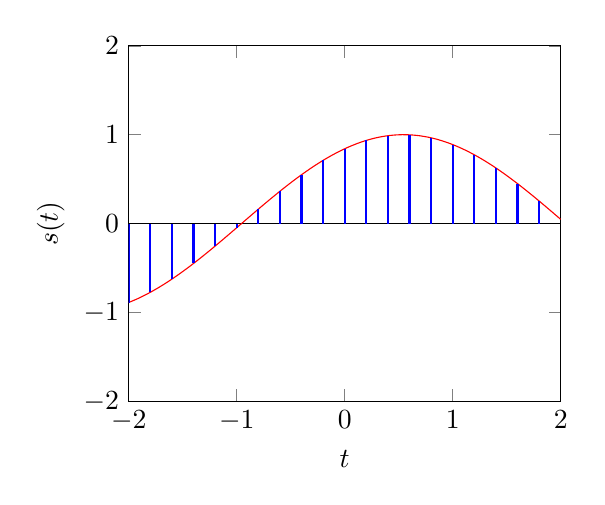
\begin{tikzpicture}
			\begin {axis}[ height = 2.4 in , xmin =-2 , xmax =2 , ymin = -2 , ymax =2 , xlabel ={$t$} , ylabel={$s(t)$} ]
			
			\addplot[domain=-2:2,samples=50,smooth,black] {0};
			\addplot[domain=-2:2,samples=50,smooth,red] {sin(deg(pi*x/3+1))};
			\addplot [ycomb , color =blue ,solid , mark options ={ solid } , thick ] plot coordinates
			{(-2.0,-0.8886510150090671) (-1.8,-0.7738868317196884) (-1.5999999,-0.6253000642942697) (-1.3999999,-0.4493846705529502) (-1.1999998,-0.25382900099061895) (-0.9999998,-0.04717984315618083) (-0.79999983,0.16153129997327936) (-0.59999985,0.3631827510192348) (-0.39999986,0.5489613749867228) (-0.19999985,0.7107477664848985) (1.4603138E-7,0.8414710674329177) (0.20000015,0.9354180471146868) (0.40000015,0.9884827666035957) (0.60000014,0.9983460455396731) (0.80000013,0.9645768168722056) (1.0000001,0.8886509577614046) (1.2000002,0.7738867526582642) (1.4000002,0.6252999668744492) (1.6000003,0.44938455903244906) (1.8000003,0.25382888024342054)};
			
		\end{axis}
	\end{tikzpicture}
\end{center}

Utilizzare il campionamento provoca una perdita di qualità del segnale.

\subsection{Interpolazione}
Fisicamente non posso far avvenire variazioni immediate del segnale (far "esplodere" il segnale); l'interpolazione ci permette di passare da segnali a tempo discreto a un segnale a tempo continuo:
$$s(t)=\sum_{n=-\infty}^{\infty}y(nT)h(t-nT)$$
con $h(t)$ risposta impulsiva dell'interpolatore.

\begin{center}
	\begin{tikzpicture}[ycomb, scale=1.5]
		\draw[->] (-3,0) -- (3,0) node[right] {$t$};
		\draw (-2,0) node[below left] {$-2T$};
		\draw (-1,0) node[below left] {$-T$};
		\draw (0,0) node[below left] {$0$};
		\draw (1,0) node[below left] {$T$};
		\draw (2,0) node[below left] {$2T$};
		\draw[color=red] plot coordinates {(-2,1) (-1,1.5) (0,-1) (1,1) (2,-0.5)};
		\draw[color=blue] (-2,0) -- (-1.7,1) -- (-1.4,0);
		\draw[color=blue] (-1,0) -- (-0.7,1.5) -- (-0.4,0);
		\draw[color=blue] (0,0) -- (0.3,-1) -- (0.6,0);
		\draw[color=blue] (1,0) -- (1.3,1) -- (1.6,0);
		\draw[color=blue] (2,0) -- (2.3,-0.5) -- (2.6,0);
	\end{tikzpicture}
\end{center}

\subsection{Holder}
L'holder ci permette di prendere un segnale discreto composto da una serie di impulsi, e allungarne gli impulsi in modo da farli durare nel tempo:
$$h(t)=rect(\frac{t-\frac{T}{2}}{T})$$
Applicando un holder a un segnale $x(nT)$ si ottiene:

\begin{center}
	\begin{tikzpicture}[ycomb, scale=1.5]
		\draw[->] (-3,0) -- (3.5,0) node[right] {$t$};
		\draw[->] (0,-1.5) -- (0,1.5) node[right] {$s(t)$};
		\draw (-2,0) node[below left] {$-2T$};
		\draw (-1,0) node[below left] {$-T$};
		\draw (0,0) node[below left] {$0$};
		\draw (1,0) node[below left] {$T$};
		\draw (2,0) node[below left] {$2T$};
		\draw (3,0) node[below left] {$3T$};
		\draw[color=red] plot coordinates {(-2,1) (-1,0.7) (0,-1) (1,1) (2,1.5)};
		\draw[color=blue] (-2,1) -| (-1,0.7);
		\draw[color=blue] (-1,0.7) -| (0,0);
		\draw[color=blue] (0,-1) -| (1,0);
		\draw[color=blue] (1,1) -| (2,1);
		\draw[color=blue] (2,1.5) -| (3,0);
	\end{tikzpicture}
\end{center}

\newpage
\subsection{Energia di un segnale}
Per un segnale a tempo continuo si ha che:
$$E_s=\int_{-\infty}^{\infty}s^2(t)dt$$
Per un segnale a tempo discreto, si usa la sommatoria $E_s=\sum_{n=-\infty}^{\infty}s^2(nT)$\\\\
Per calcolare l'energia di un segnale attenuato abbiamo che:
$$E_{(As(t))}=A^2E_s$$

\subsection{Segnali in decibel}
Per passare l'energia di un segnale in decibel si usa il seguente passaggio:
$$(E_s)_{dB}=10\log(E_s)$$

\subsection{Spazio vettoriale di segnali a energia finita}

\subsubsection{Prodotto interno}
Definiamo il prodotto interno tra due vettori come:
$$\langle\;x(t),\;y(t)\;\rangle=\int_{-\infty}^{\infty}x(t)y(t)\;dt$$

\subsubsection{Norma di un vettore}
Definiamo la norma di un vettore come:
$$||s(t)||=\sqrt{\langle\;s(t),\;s(t)\;\rangle}=\sqrt{E_s}$$

\subsubsection{Base ortonormale}
una base ortonormale di uno spazio vettoriale è un insieme di vettori $\phi_1(t),...,\phi_I(t)$ tali che:
$$\begin{array}{rcrcrc}
	\langle\;x_i(t),\;x_j(t)\;\rangle=0,& i\neq j,\;\forall\;i,j\\\\
	||x_i(t)||=1,&\forall\;i
\end{array}$$
Deve inoltre valere che un segnale generico $y(t)$ sia scrivibile come combinazione lineare dei vettori della base:
$$y(t)=\sum_ {n=1}^I\langle\;y(t),\;x_n(t)\;\rangle x_n(t)$$
I vettori della base sono \textbf{ortogonali} in quanto il loro prodotto interno fa 0 e \textbf{normali} in quando il modulo di ognuno di loro vale 1.\\\\
Da notare che due vettori sono ortogonali in due casi:
\begin{enumerate}
	\item se i due segnali hanno \textbf{sostegni diversi}:
	\begin{center}
		\begin{tikzpicture}
			\draw[->] (-0.2,0) -- (4,0) node[right] {$t$};
			\draw[->] (0,-0.2) -- (0,1.5) node[right] {$x(t)$};
			\draw[color=red] (0,0) |- (1,1) -- (1,0);
			
			\draw[->] (-0.2,-3) -- (4,-3) node[right] {$t$};
			\draw[->] (0,-3.2) -- (0,-1.5) node[right] {$y(t)$};
			\draw[color=red] (1.5,-3) -- (2,-2) -- (2.5,-3);
			\foreach \x in {1, 1.5, 2.5} \draw[dotted] (\x,-3) -- (\x,0);
		\end{tikzpicture}
	\end{center}
	\item se l'area del prodotto dei due segnali è nulla
	\begin{center}
		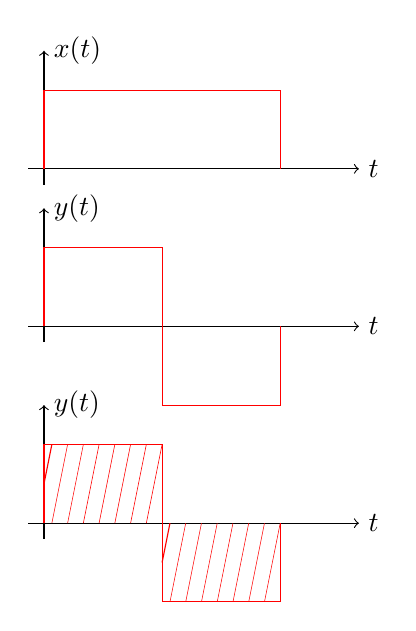
\begin{tikzpicture}
			\draw[->] (-0.2,0) -- (4,0) node[right] {$t$};
			\draw[->] (0,-0.2) -- (0,1.5) node[right] {$x(t)$};
			\draw[color=red] (0,0) |- (1.5,1) -| (3,0);
			\draw[->] (-0.2,-2) -- (4,-2) node[right] {$t$};
			\draw[->] (0,-2.2) -- (0,-0.5) node[right] {$y(t)$};
			\draw[color=red] (0,-2) |- (1.5,-1) -- (1.5,-3) -| (3,-2);
			\draw[->] (-0.2,-4.5) -- (4,-4.5) node[right] {$t$};
			\draw[->] (0,-4.7) -- (0,-3) node[right] {$y(t)$};
			\draw[color=red] (0,-4.5) |- (1.5,-3.5) -- (1.5,-5.5) -| (3,-4.5);
			\draw[color=red] (0,-4) -- (0.1, -3.5);
			\foreach \x in {0.1, 0.3, 0.5, 0.7, 0.9, 1.1, 1.3} \draw[color=red, very thin] (\x, -4.5) -- (\x+0.2, -3.5);
			\draw[color=red] (1.5,-5) -- (1.6, -4.5);
			\foreach \x in {1.6, 1.8, 2, 2.2, 2.4, 2.6, 2.8} \draw[color=red, very thin] (\x, -5.5) -- (\x+0.2, -4.5);
		\end{tikzpicture}
	\end{center}
\end{enumerate}

\subsubsection{Metodo di orto normalizzazione di Gram Schmidt}
Supponiamo di avere N vettori $s_1(t),...,s_N(t)$ e vogliamo trovare una base ortonormale per questi vettori: il primo passo è scegliere uno dei vettori e \textbf{normalizzarlo}, per usarlo come primo vettore della base:
$$\phi_1(t)=\frac{s_i(t)}{\sqrt{E_{s_1}}}$$
Ora dobbiamo trovare gli altri vettori della base con il seguente processo:
$$\phi_i'(t)=s_j(t)-\sum_{k=1}^{i-1}\langle\;s_k(t),\;\phi_i(t)\;\rangle\;\phi_i(t)$$
Ripetiamo quindi il processo finché non troviamo una base completa per i vettori dati.









\newpage
\section{Modulazione digitale}

\subsection{Ricevitore digitale}
Il ricevitore digitale rappresenta un segnale ricevuto nello spazio della costellazione.\\
Un segnale trasmesso in un canale AWGN, sarà ricevuto nella seguente forma:
$$r(t)=s_{a_n}(t)+w(t)$$
$s_{a_n}(t)$ è il simbolo che era stato trasmesso, mentre $w(t)$ è il \textbf{rumore che è stato introdotto dal canale}.\\
Il messaggio ricevuto è ovviamente una sequenza di simboli, i quali sono ricavabili applicando un ritardo di $nT$ ai segnali.

\subsection{Il rumore dopo la proiezione}
Se trasmettiamo in un canale AWGN, il rumore è rappresentabile come una \textbf{v.a. Gaussiana} a media nulla e varianza indipendente dal rumore in altri istanti.
$$w(t)\sim N(0,\sigma_w^2)$$
Avendo media nulla, \textbf{l'energia del rumore si può approssimare a 0}.\\

\subsection{Regioni di decisione}
Per via del rumore, non sono certo di ricevere esattamente i simboli che vengono trasmessi, di conseguenza ho bisogno di determinare dei criteri per scegliere un segnale piuttosto che un altro, dato un segnale ricevuto.\\
Devo trovare un metodo per dividere lo spazio in $M$ regioni, in modo da esaurire l'intero spazio euclideo, e non avere zone di indecisioni.
\begin{center}
	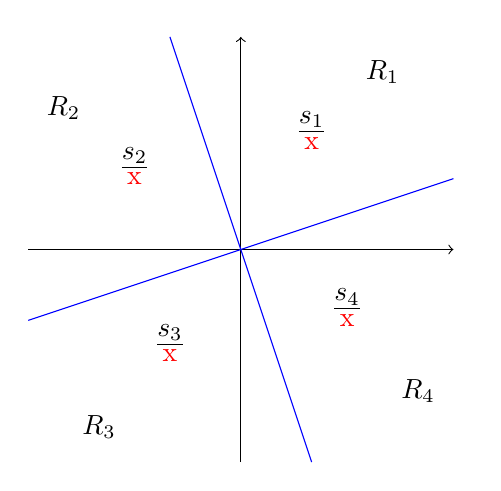
\begin{tikzpicture}[scale=0.9]
		\draw[->] (-3,0) -- (3,0) node[right]{};
		\draw[->] (0,-3) -- (0,3) node[right]{};
		\draw[color=blue] (-1, 3) -- (1,-3);
		\draw[color=blue] (-3, -1) -- (3,1);
		\node[red] at (1,1.5){x};
		\node[above] at (1,1.5){$\underline{s_1}$};
		\node[red] at (-1.5,1){x};
		\node[above] at (-1.5,1){$\underline{s_2}$};
		\node[red] at (-1,-1.5){x};
		\node[above] at (-1,-1.5){$\underline{s_3}$};
		\node[red] at (1.5,-1){x};
		\node[above] at (1.5,-1){$\underline{s_4}$};
		\node at (2,2.5){$R_1$};
		\node at (-2.5,2){$R_2$};
		\node at (-2,-2.5){$R_3$};
		\node at (2.5,-2){$R_4$};
	\end{tikzpicture}
\end{center}
Per scegliere quale regione utilizzare, usiamo la \textbf{probabilità di decisione corretta}.

\subsection{Probabilità di decisione corretta}
Non sempre il ricevitore farà la decisione corretta, dobbiamo quindi calcolare la probabilità che il ricevitore la faccia:
$$P(C)=\sum_{n=1}^N\biggl(\int_{\Re_n}p_{r|a_0}(r|n)P_{a_0}(n)dr\biggl)$$
$N$ è il numero di regioni di decisione, $\Re_n$ è la n-esima regione di decisione, $p_{r|a_0}(r|n)$ è la densità di probabilità del rumore per un dato simbolo, $P_{a_0}(n)$ è la probabilità di trasmissione del simbolo $n$.
Il mio scopo è massimizzare la probabilità di decisione corretta: esistono vari criteri:
\begin{enumerate}
	\item \textbf{MAP}: $a_0=argmax_n\biggl(p_{a_0|n}(n|r)\biggl)$ da usare in caso generico
	\item \textbf{ML}: $a_0=argmax_n\biggl(p_{r|a_0}(r|n)\biggl)$ da usare quando i simboli trasmessi sono equiprobabili
	\item \textbf{MD}: $a_0=argmin_n\biggl(d^2(r, s_n)\biggl)$ da usare se si hanno simboli equiprobabili trasmessi in un canale AWGN
\end{enumerate}

\subsection{Ricevitori digitali}
\begin{enumerate}
	\item \textbf{MAP-ML}
	\begin{center}
		%%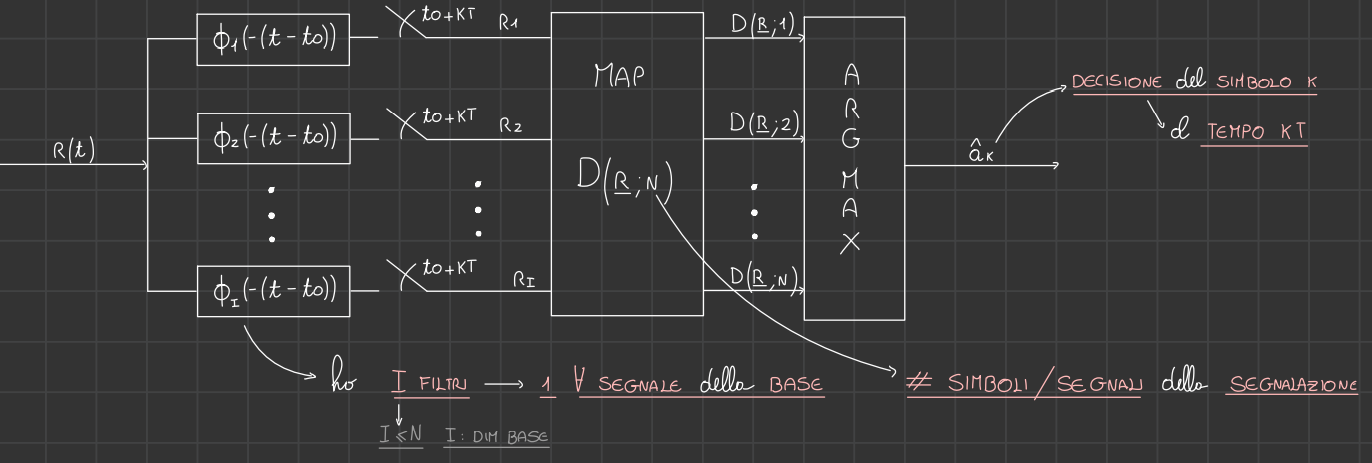
\includegraphics[scale=0.23]{img/FDT--2022-10-25--02.png}
	\end{center}
	\item \textbf{MD-1}
	\begin{center}
		%%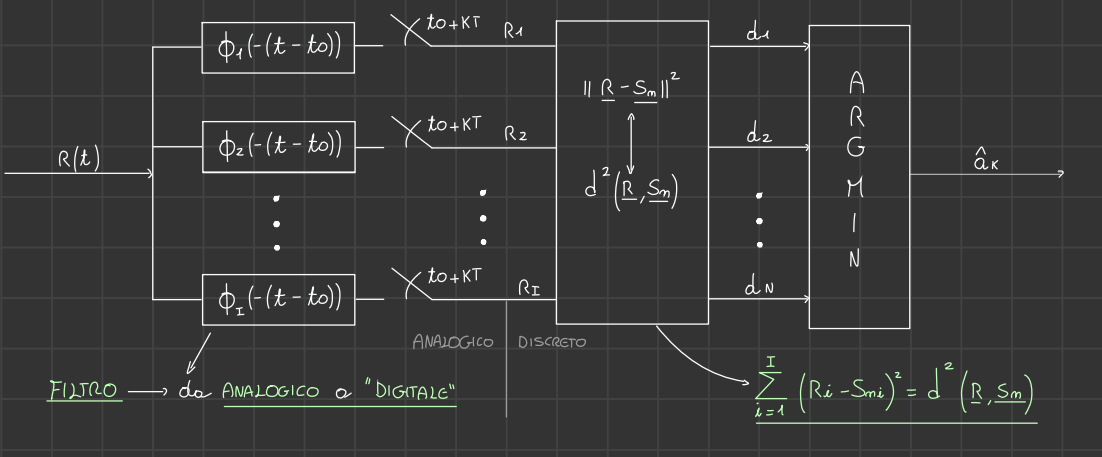
\includegraphics[scale=0.25]{img/FDT--2022-10-25--03.png}
	\end{center}
	\item \textbf{MD-2}
	\begin{center}
		%%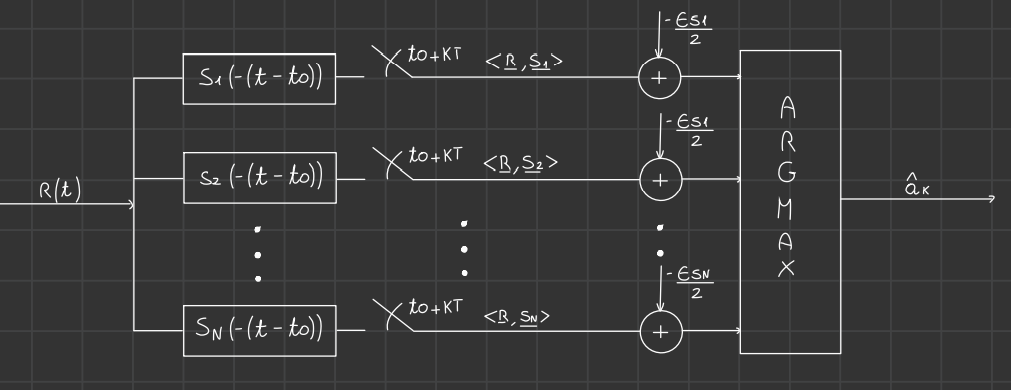
\includegraphics[scale=0.28]{img/FDT--2022-10-25--04.png}
	\end{center}
\end{enumerate}

\subsection{Modulazione binaria}
Nella modulazione binaria abbiamo \textbf{due simboli} ($M=2$) che mappano i valori di un bit.
Sia $I$ la dimensione della base:
\begin{enumerate}
	\item \textbf{I=1}:
	\begin{center}
		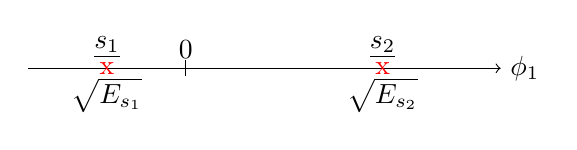
\begin{tikzpicture}
			\draw[->] (-3,0) -- (3,0) node[right]{$\phi_1$};
			\node[red] at (-2,0){x};
			\node[above] at (-2,0){$\underline{s_1}$};
			\node[below] at (-2,0){$\sqrt{E_{s_1}}$};
			\node[above] at (-1,0) {$0$};
			\draw[color=black] (-1,-0.1) -- (-1,0.1);
			\node[red] at (1.5,0){x};
			\node[above] at (1.5,0){$\underline{s_2}$};
			\node[below] at (1.5,0){$\sqrt{E_{s_2}}$};
		\end{tikzpicture}
	\end{center}
	\item \textbf{I=2}:
	\begin{center}
		\begin{tikzpicture}
			\draw[->] (-3,0) -- (3,0) node[right]{$\phi_1$};
			\draw[->] (0,-0.5) -- (0,3) node[right]{$\phi_2$};
			\node[red] at (2,2){x};
			\node[right] at (2,2){$\underline{s_1}$};
			\node[red] at (-1,1){x};
			\node[left] at (-1,1){$\underline{s_2}$};
			\draw[dotted] (-1,1) -- (0,0) -- (2,2);
		\end{tikzpicture}
	\end{center}
	$$|\underline{s_i}|=\sqrt{E_{s_i}}$$
\end{enumerate}
Nel caso di una base a due vettori si ha che
$$\begin{array}{c}
	\underline{s_1}=\biggl[\langle\;s_1(t),\;\phi_1(t)\;\rangle,\langle\;s_1(t),\;\phi_2(t)\;\rangle\biggl]\\\\
	\underline{s_2}=\biggl[\langle\;s_2(t),\;\phi_1(t)\;\rangle,\langle\;s_2(t),\;\phi_2(t)\;\rangle\biggl]
\end{array}$$

\subsubsection{Probabilità d'errore}
$$P(E)=Q\biggl(\frac{d}{2\sigma_I}\biggl)$$
$Q(A)$ mi rappresenta l'area della gaussiana per i valori $>A$\\
Per diminuire la probabilità d'errore bisogna aumentare la distanza tra i vettori o trovare un modo per diminuire la varianza del rumore.

\subsubsection{Energia media della modulazione}
$$E_s=E\biggl[E_{s_i}\biggl]=\sum_{i=1}^ME_{s_i}P_{a_0}(i)$$
L'energia media è il valore atteso delle energie dei simboli.\\

\subsubsection{Coefficiente di correlazione}
$$\rho=\frac{\langle\;\underline{s}_1,\;\underline{s}_2\;\rangle}{\sqrt{E_{s_1},E_{s_2}}}$$
Se $\rho=0$ il prodotto interno è nullo, quindi i due segnali sono ortogonali.\\
Se $\rho=-1$ è possibile (non è per forza vero) che i segnali siano antipodali; perché i segnali lo siano devono anche essere opposti ($s_1(t)=-s_2(t)$).\\
Sfruttando il coefficiente di correlazione ci è possibile trovare le coordinate dei segnali anche senza conoscere la base della segnalazione:
$$\begin{array}{c}
	\underline{s_1}=\biggl[\sqrt{E_{s_1}},0\biggl]\\\\
	\underline{s_2}=\biggl[\rho\sqrt{E_{s_2}},\sqrt{E_{s_2}}\sqrt{1-\rho^2}\biggl]
\end{array}$$

\subsection{Modulazioni M-arie}
In generale, se abbiamo una segnalazione di \textbf{dimensione M}, valgono le seguenti regole:

\subsubsection{Probabilità d'errore}
\begin{enumerate}
	\item \textbf{Limite inferiore}:$$P(E)\geq\frac{1}{M}\sum_{m=1}^MQ\biggl(\frac{d_{min}}{2\sigma_I}\biggl)$$
	\item \textbf{Limite superiore}:$$P(E)\leq(m-1)Q\biggl(\frac{d_{min}}{2\sigma_I}\biggl)$$
	\item \textbf{Modulazione ortogonale}:$$\frac{M+1}{2}Q\biggl(\sqrt{\frac{E_s}{2\sigma_I^2}}\biggl)\leq P(E)\leq(M-1)Q\biggl(\sqrt{\frac{E_s}{2\sigma_I^2}}\biggl)$$
	\item \textbf{Modulazione bi-ortogonale}:$$\frac{M-1}{2}Q\biggl(\sqrt{\frac{E_s}{2\sigma_I^2}}\biggl)+\frac{1}{M}Q\biggl(\sqrt{\frac{E_s}{\sigma_I^2}}\biggl)\leq P(E)\leq(M-2)Q\biggl(\sqrt{\frac{E_s}{2\sigma_I^2}}\biggl)+Q\biggl(\sqrt{\frac{E_s}{\sigma_I^2}}\biggl)$$
\end{enumerate}

\subsection{Modulazione PAM}
Nella modulazione PAM abbiamo un segnale base $h_{TX}(t)$ usato come base, \textbf{scalato poi  M volte}:
\begin{center}
	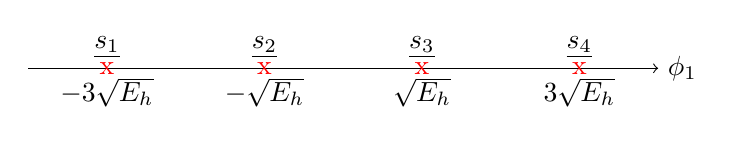
\begin{tikzpicture}
		\draw[->] (-4,0) -- (4,0) node[right]{$\phi_1$};
		\foreach \x in {-3,-1,1,3} \node[red] at (\x,0){x};
		\node[above] at (-3,0){$\underline{s_1}$};
		\node[above] at (-1,0){$\underline{s_2}$};
		\node[above] at (1,0){$\underline{s_3}$};
		\node[above] at (3,0){$\underline{s_4}$};
		\node[below] at (-3,0){$-3\sqrt{E_{h}}$};
		\node[below] at (-1,0){$-\sqrt{E_{h}}$};
		\node[below] at (1,0){$\sqrt{E_{h}}$};
		\node[below] at (3,0){$3\sqrt{E_{h}}$};
	\end{tikzpicture}
\end{center}
$$s_m(t)=\alpha_mh_{TX}(t)\qquad\alpha_m=2m-1-M,\quad m\in[1,M]$$
la base ha dimensione 1 e $\phi(t)=\frac{h_{TX}(t)}{\sqrt{E_h}}$.\\
La distanza tra due simboli adiacenti è di $2\sqrt{E_h}$.\\

\subsubsection{Simboli}
$$\underline{s_m}=\alpha_m\sqrt{E_h}$$

\subsubsection{Energia media}
$$E_s=\frac{M^2-1}{3}E_h$$

\subsubsection{Probabilità d'errore}
Analizzando una sezione per volta, notiamo due tipi di regioni di decisione: una esterna e una interna.
\begin{enumerate}
	\item \textbf{Regione interna}:$$P(E)=Q\biggl(\sqrt{\frac{E_h}{\sigma_I^2}}\biggl)$$
	\item \textbf{Regione interna}:$$P(E)=2Q\biggl(\sqrt{\frac{E_h}{\sigma_I^2}}\biggl)$$
\end{enumerate}
Andando a calcolare la probabilità d'errore totale abbiamo che, se i simboli sono trasmessi con la stessa probabilità:$$P(E)=2\frac{M-1}{M}Q\biggl(\sqrt{\frac{E_s}{\sigma_I^2}}\biggl)$$\\
Utilizzando poi la mappatura di Gray per mappare i bit all'interno della segnalazione (due simboli diversi possono differire solo di un bit), otteniamo che la probabilità d'errore sul bit è di $P_{bit}=\frac{P(E)}{\log_2(M)}$

\subsection{Modulazione QAM}
La modulazione QAM è simile alla PAM, solo che si sviluppa su una base di dimensione 2:
\begin{center}
	\begin{tikzpicture}
		\draw[->] (-4,0) -- (4,0) node[right]{$\phi_1$};
		\draw[->] (0,-4) -- (0,4) node[right]{$\phi_2$};
		\node[above] at (-3, 0){$-3\sqrt{E_h}$};
		\node[above] at (-1, 0){$-\sqrt{E_h}$};
		\node[above] at (1, 0){$\sqrt{E_h}$};
		\node[above] at (3, 0){$3\sqrt{E_h}$};
		\node[above left] at (0, -3){$-3\sqrt{E_h}$};
		\node[above left] at (0, -1){$-\sqrt{E_h}$};
		\node[above left] at (0, 1){$\sqrt{E_h}$};
		\node[above left] at (0, 3){$3\sqrt{E_h}$};
		\foreach \x in {-3,-1,1,3}
		\draw (\x, -0.1) -- (\x, 0.1);
		\foreach \x in {-3,-1,1,3}
		\draw (-0.1, \x) -- (0.1, \x);
		\foreach \x in {-3,-1,1,3}
		\foreach \x in {-3,-1,1,3}
		\node[color=red] at (\x,-3){x};
		\foreach \x in {-3,-1,1,3}
		\node[color=red] at (\x,-1){x};
		\foreach \x in {-3,-1,1,3}
		\node[color=red] at (\x,1){x};
		\foreach \x in {-3,-1,1,3}
		\node[color=red] at (\x,3){x};
	\end{tikzpicture}\\
	esempio di una 16-QAM
\end{center}
$$\begin{array}{c}
	s_m(t)=\alpha_{m,I}\;h_{TX}(t)\cos(2\pi f_0t+\varphi_0)-\alpha_{m,Q}\;h_{TX}(t)\sin(2\pi f_0t+\varphi_0)\\\\
	\alpha_{m,I},\alpha_{m,Q}=2l-L-1\;\;\;m\in[1,M],\;l=\sqrt{M}
\end{array}$$

\subsubsection{Base}
Abbiamo come base per la segnalazione:
$$\begin{array}{c}
	\phi_1(t)=\sqrt{2\over E_{ h_{TX}}}\cos(2\pi f_0t+\varphi_0)h_{TX}(t)\\\\
	\phi_1(t)=-\sqrt{2\over E_{ h_{TX}}}\sin(2\pi f_0t+\varphi_0)h_{TX}(t)
\end{array}$$

\subsubsection{Simboli}
$$\underline{s_m}=\biggl[\sqrt{\frac{E_h}{2}}\alpha_{m,I},\sqrt{\frac{E_h}{2}}\alpha_{m,Q}\biggl]$$

\subsubsection{Energia media}
$$E_s=\frac{M-1}{3}E_h$$

\subsubsection{Probabilità d'errore}

\begin{center}
	\begin{tikzpicture}[scale=0.9]
		\draw[->] (-4,0) -- (4,0) node[right]{$\phi_1$};
		\draw[->] (0,-4) -- (0,4) node[right]{$\phi_2$};
		\foreach \x in {-2, 2} \draw (\x, -3.7) -- (\x, 3.7);
		\foreach \x in {-2, 2} \draw (-3.7, \x) -- (3.7, \x);
		\foreach \x in {-3,-1,1,3}
		\draw (\x, -0.1) -- (\x, 0.1);
		\foreach \x in {-3,-1,1,3}
		\draw (-0.1, \x) -- (0.1, \x);
		\foreach \x in {-3,-1,1,3}
		\foreach \x in {-3,-1,1,3}
		\node[color=red] at (\x,-3){x};
		\foreach \x in {-3,-1,1,3}
		\node[color=red] at (\x,-1){x};
		\foreach \x in {-3,-1,1,3}
		\node[color=red] at (\x,1){x};
		\foreach \x in {-3,-1,1,3}
		\node[color=red] at (\x,3){x};
	\end{tikzpicture}
\end{center}

Analizzando una sezione per volta, notiamo 3 tipi di regioni di decisione: una interna, una sugli angoli e una sui lati.
\begin{enumerate}
	\item \textbf{Regione sugli angoli}:$$P(C|A)=\biggl(1-Q\biggl(\sqrt{\frac{E_h}{2\sigma_I^2}}\biggl)\biggl)^2$$
	\item \textbf{Regione sui lati}:$$P(C|B)=\biggl(1-2Q\biggl(\sqrt{\frac{E_h}{2\sigma_I^2}}\biggl)\biggl)\biggl(1-Q\biggl(\sqrt{\frac{E_h}{2\sigma_I^2}}\biggl)\biggl)$$
	\item \textbf{Regione centrale}:$$P(C|C)=\biggl(1-2Q\biggl(\sqrt{\frac{E_h}{2\sigma_I^2}}\biggl)\biggl)^2$$
\end{enumerate}
Andando a calcolare la probabilità d'errore totale abbiamo che, se i simboli sono trasmessi con la stessa probabilità:
$$P(E)=4(\frac{L-1}{L})Q\biggl(\sqrt{\frac{3/2}{M-1}\frac{E_s}{\sigma_I^2}}\biggl)$$
Utilizzando poi la mappatura di Gray per mappare i bit all'interno della segnalazione (due simboli diversi possono differire solo di un bit), otteniamo che la probabilità d'errore sul bit è di $P_{bit}=\frac{P(E)}{\log_2(M)}$

\subsection{Quantizzazione}
La quantizzazione è un processo che trasforma un segnale $y(kT)\in\Re$ in $y_q(kT)\in A$, con $A$ un alfabeto di valori discreti.

\subsubsection{Funzione caratteristica}
La funzione caratteristica di un quantizzatore indica i valori quantizzati in base al valore reale $y(t)$:
\begin{center}
	\begin{tikzpicture}
		\draw[->] (-2,0) -- (4,0) node[right]{$y$};
		\draw[->] (0,-1) -- (0,3) node[right]{$y_a$};
		\draw[color=red] (-2,-0.5) -- (-0.5,-0.5);
		\draw[color=red] (-0.5,0.2) -- (0.2,0.2);
		\draw[color=red] (0.2,2) -- (1.5,2);
		\draw[color=red] (1.5,1.5) -- (2,1.5);
		\draw[color=red] (2,2.7) -- (4,2.7);
		\draw[dotted] (-0.5,-0.5) -- (-0.5,0.2);
		\draw[dotted] (0.2,0.2) -- (0.2,2);
		\draw[dotted] (1.5,2) -- (1.5,1.5);
		\draw[dotted] (2,1.5) -- (2,2.7);
		\foreach \x in {-0.5, 0.2, 1.5, 2, 2.7} \draw (-0.1, \x) -- (0.1,\x);
		\node[above left] at (0, -0.5){$a_1$};
		\node[above left] at (0, 0.2){$a_2$};
		\node[above left] at (0, 1.5){$a_3$};
		\node[above left] at (0, 2){$a_4$};
		\node[above left] at (0, 2.7){$a_5$};
	\end{tikzpicture}
\end{center}

\subsubsection{Quantizzatore uniforme}
La funzione caratteristica di un quantizzatore uniforme è la seguente:
\begin{center}
	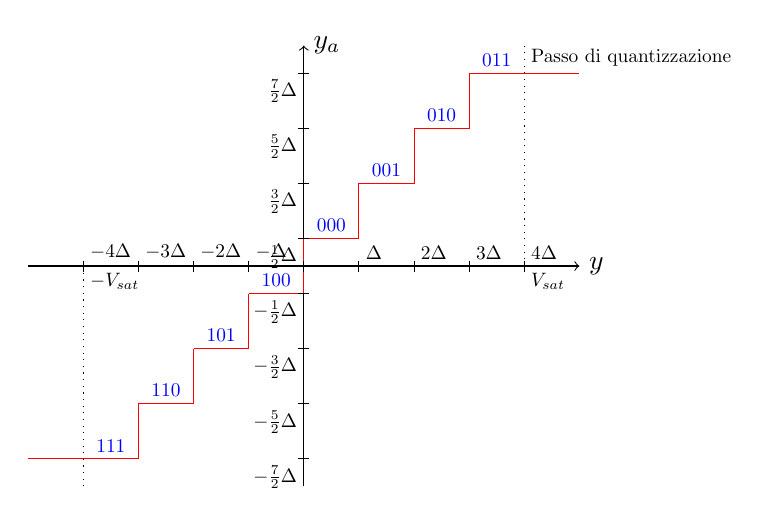
\begin{tikzpicture}[scale=0.7]
		\draw[->] (-5,0) -- (5,0) node[right]{$y$};
		\draw[->] (0,-4) -- (0,4) node[right]{$y_a$};
		\foreach \x in {-4,-3,-2,-1,0,1,2} \draw[color=red] (\x, \x+1/2) -| (\x+1, \x+3/2);
		\draw[color=red] (-5,-7/2) -- (-4,-7/2);
		\draw[color=red] (3,7/2) -- (5,7/2);
		\node[above, color=blue, scale=0.7] at (-3.5, -7/2){$111$};
		\node[above, color=blue, scale=0.7] at (-2.5, -5/2){$110$};
		\node[above, color=blue, scale=0.7] at (-1.5, -3/2){$101$};
		\node[above, color=blue, scale=0.7] at (-0.5, -1/2){$100$};
		\node[above, color=blue, scale=0.7] at (0.5, 1/2){$000$};
		\node[above, color=blue, scale=0.7] at (1.5, 3/2){$001$};
		\node[above, color=blue, scale=0.7] at (2.5, 5/2){$010$};
		\node[above, color=blue, scale=0.7] at (3.5, 7/2){$011$};
		\foreach \x in {-4,-3,-2,-1,0,1,2,3,4} \draw (\x, 0.1) -- (\x, -0.1);
		\foreach \x in {-7/2,-5/2,-3/2,-1/2,1/2,3/2,5/2,7/2} \draw (0.1, \x) -- (-0.1, \x);
		\node[scale=0.7, above right] at (-4, 0){$-4\Delta$};
		\node[scale=0.7, below right] at (-4, 0){$-V_{sat}$};
		\node[scale=0.7, above right] at (-3, 0){$-3\Delta$};
		\node[scale=0.7, above right] at (-2, 0){$-2\Delta$};
		\node[scale=0.7, above right] at (-1, 0){$-\Delta$};
		\node[scale=0.7, above right] at (1, 0){$\Delta$};
		\node[scale=0.7, above right] at (2, 0){$2\Delta$};
		\node[scale=0.7, above right] at (3, 0){$3\Delta$};
		\node[scale=0.7, above right] at (4, 0){$4\Delta$};
		\node[scale=0.7, below right] at (4, 0){$V_{sat}$};
		\node[scale=0.7, below left] at (0, 7/2){$\frac{7}{2}\Delta$};
		\node[scale=0.7, below left] at (0, 5/2){$\frac{5}{2}\Delta$};
		\node[scale=0.7, below left] at (0, 3/2){$\frac{3}{2}\Delta$};
		\node[scale=0.7, below left] at (0, 1/2){$\frac{1}{2}\Delta$};
		\node[scale=0.7, below left] at (0, -1/2){$-\frac{1}{2}\Delta$};
		\node[scale=0.7, below left] at (0, -3/2){$-\frac{3}{2}\Delta$};
		\node[scale=0.7, below left] at (0, -5/2){$-\frac{5}{2}\Delta$};
		\node[scale=0.7, below left] at (0, -7/2){$-\frac{7}{2}\Delta$};
		\draw[dotted] (-4,-4) -- (-4, 0);
		\draw[dotted] (4,0) -- (4,4);
		\node[above right, scale = 0.7] at (4, 7/2){Passo di quantizzazione};
	\end{tikzpicture}
\end{center}
$$\Delta=\frac{2V_{sat}}{L}$$
$\Delta$ è detto passo di quantizzazione, $L$ è il numero di livelli ($L=2^b$, b numero di bit).\\\\
In un quantizzatore possiamo trovare due tipi di errori:
\begin{enumerate}
	\item \textbf{Errore granulare}: Quando $y\in[-V_{sat},V_{sat}]$
	\item \textbf{Errore di saturazione}: Quando $y\not\in[-V_{sat},V_{sat}]$
\end{enumerate}

\subsubsection{Gestione dell'errore di saturazione}
Abbiamo due casi da distinguere:
\begin{enumerate}
	\item Se il segnale è \textbf{limitato} in $[-A,A]$ scelgo un $V_{sat}$ in modo che $V_{sat}=A$ per evitare un errore di saturazione
	\item Se il segnale ha una \textbf{densità di probabilità con supporto non finito}, non posso impedire la saturazione;\\
	Scelgo una probabilità di saturazione che soddisfi le mie necessità, e calcolo $V_{sat}$ di conseguenza:$$P(y\not\in[-V_{sat},V_{sat}])\leq P_{sat}$$
\end{enumerate}

\subsubsection{Gestione dell'errore granulare}
\begin{center}
	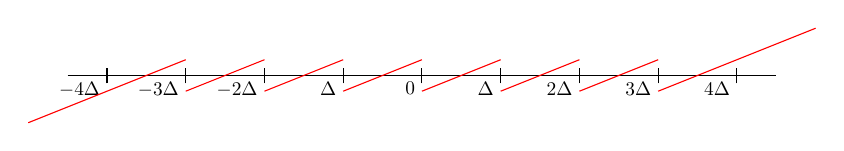
\begin{tikzpicture}
		\draw (-4.5, 0) -- (4.5, 0);
		\foreach \x in {-4,-3,-2,-1,0,1,2,3,4} \draw (\x, -0.1) -- (\x, 0.1);
		\node[below left, scale=0.7] at (-4,0){$-4\Delta$};
		\node[below left, scale=0.7] at (-3,0){$-3\Delta$};
		\node[below left, scale=0.7] at (-2,0){$-2\Delta$};
		\node[below left, scale=0.7] at (-1,0){$\Delta$};
		\node[below left, scale=0.7] at (0,0){$0$};
		\node[below left, scale=0.7] at (1,0){$\Delta$};
		\node[below left, scale=0.7] at (2,0){$2\Delta$};
		\node[below left, scale=0.7] at (3,0){$3\Delta$};
		\node[below left, scale=0.7] at (4,0){$4\Delta$};
		\foreach \x in {-4,-3,-2,-1,0,1,2,3} \draw[red] (\x,-0.2) -- (\x+1, 0.2);
		\draw[red] (-5, -0.6) -- (-4,-0.2);
		\draw[red] (4,0.2) -- (5,0.6);
	\end{tikzpicture}
\end{center}
$$e_q=y-y_a$$\\
L'errore granulare, ha valori all'interno dell'intervallo $e_q\in[-\Delta/2;\Delta/2]$.
Supponendo di avere un numero $L$ di livelli alto, $\Delta$ assumerà un valore piccolo.
$$P_y(a)\simeq P_y(a_i)\qquad a\in[a_i-\frac{\Delta}{2},a_i+\frac{\Delta}{2}]$$
Supponendo che $e_q$ sia uniforme in $[-\Delta/2,\Delta/2]$, si ha che il valore atteso dell'errore granulare è 0 $E[e_q]=0$ mentre la varianza è $\sigma_y=\frac{\Delta^2}{12}$

\subsubsection{Rapporto segnale-rumore}
$$(\Lambda)_{dB}=20\log(\frac{\sigma_y}{V_{sat}})+4.77+6.02b$$
Aumentare il numero di bit utilizzati, aumenta di 6 il SNR (Signal Noise Ratio).











\newpage
\section{Struttura dei sistemi di comunicazione}
I sistemi di comunicazione coinvolgono \textbf{più tipi di dispositivi connessi}.\\
Non c'è più una comunicazione punto punto, ma esiste una comunicazione tra più dispositivi.\\\\
Ci sono due concetti principali quando si parla di sistemi di comunicazione:
\begin{enumerate}
	\item \textbf{Piano di controllo}: insieme delle procedure, tecniche e hardware necessario per il funzionamento di una rete
	\item \textbf{Piano dei dati}: comunicazione dei dati dell'utente
\end{enumerate}

\subsection{Protocolli di comunicazione}
Un protocollo di comunicazione è un insieme di regole per lo scambio dei messaggi tra più dispositivi.

\subsubsection{Standard OSI}
Da' un quadro generale per creare uno standard di comunicazione.\\
Lo \textbf{standard OSI} separa uno standard di telecomunicazione in 7 strati.\\
Ogni strato di un dispositivo A deve comunicare con il rispettivo strato di un dispositivo B, attraversando tutti gli strati inferiori.
\begin{enumerate}
	\item \textbf{Fisico}: Si occupa della trasmissione dei dati su uno specifico mezzo di comunicazione
	\item \textbf{Collegamento dati}: Creare una comunicazione affidabile e coordinare la trasmissione tra più dispositivi (migliorare e tenere sotto controllo gli errori che possono avvenire nello strato fisico)
	\item \textbf{Rete}: Si occupa dell'instradamento: non siamo più in situazione di punto punto, ma serve inviare messaggi attraverso dispositivi diversi prima di raggiungere la destinazione finale
	\item \textbf{Trasporto}: Rende affidabile il collegamento end-to-end nella rete
	\item \textbf{Sessione}:Stabilisce il periodo nel quale due entità di parlano tra loro;\\
	Si stabiliscono delle regole (es attivare e disattivare canali di comunicazione per parlare a turni)
	\item \textbf{Presentazione}: Troviamo ciò che riguarda il contenuto del messaggio
	\item \textbf{Applicazione}: Gestione completa dell'applicazione/del servizio
\end{enumerate}

\subsection{Codifica di canale}
Tecniche che ci permettono di \textbf{rendere affidabile} la comunicazione e correggere (in parte) gli errori sul bit.\\
Ci sono due strategie generali:
\begin{enumerate}
	\item \textbf{Ritrasmissione}\\
	chiediamo al mittente di \textbf{ripetere} un messaggio;\\
	dobbiamo essere in grado di capire se c'è stato un errore e dobbiamo essere in grado di poter comunicare al mittente la richiesta di ritrasmissione
	\item \textbf{Codifica del messaggio in trasmissione}\\
	elaboro la sequenza di bit (aggiungo dei bit) calcolati sui bit del messaggio, che mi aiutano di \textbf{correggere alcuni errori} (es bit di parità);\\
	Questa tecnica mi allunga il pacchetto di bit, e c'è una possibilità di non dover utilizzare questi bit (nel caso non ci siano stati errori)
\end{enumerate}
Ci sarebbe anche una terza strategia ibrida: una ritrasmissione in cui vengono mandati solo dei bit di codifica.

\subsection{Canale Binario}
Abbiamo un canale binario che trasmette dei bit $c_k\in\{0,1\}$; il ricevitore tuttavia riceve dei bit $\hat{c_k}\in\{0,1\}$ non per forza uguali ai bit trasmessi.\\
Il canale binario può essere rappresentato come una serie di un modulatore digitale, un canale (es AWGN) e un demodulatore digitale.\\
Nel caso in cui la probabilità di sbagliare un bit invece che un altro, si dice che ci troviamo in un \textbf{canale binario simmetrico senza memoria}.
$$P(\hat{c_k}=1|c_k=0)=P(\hat{c_k}=0|c_k=1)=P_{bit}$$
Inoltre, in un canale del genere, gli errori su bit distinti sono indipendenti.\\
Attenzione che non tutti i canali binaria si comportano in questo modo, è una situazione ideale ma che ci semplificherà i calcoli e le analisi dei canali.\\
Il modello a cui facciamo riferimento per correggere gli errori è quello dei \textbf{codici di canale a blocco}.

\subsubsection{Codici di canale a blocco}
A partire da blocchi di $k$ bit, generiamo blocchi di $n$ bit, con $n>k$ (sia $k$ che $n$ saranno nomi di variabili riservate a queste nozioni).\\
I blocchi di ingresso (lunghi $k$) contengono il messaggio che vogliamo trasmettere, quelli di uscita includono anche un'informazione per correggere gli errori.\\
$$\underline{b}=[b_1,...,b_k]\rightarrow\underline{c}=[c_1,...,c_n]\rightarrow\mbox{CAN BIN}\rightarrow\underline{\hat{c}}=[\hat{c_1},...,\hat{c_n}]\rightarrow\underline{\hat{b}}=[\hat{b_1},...,\hat{b_k}]$$
I possibili vettori $\underline{b}$ in ingresso sono $2^k$; i possibili messaggi $\underline{c}$ che escono dal codificatore sono comunque $2^k$, in quanto il numero di messaggi codificati è pari al numero di messaggi da codificare, i quali sono $2^k$.\\
Al ricevitore invece, per via dei disturbi all'interno del canale, ricevo $2^n$ messaggi $\underline{\widetilde{c}}$ da decodificare, i quali diventeranno di nuovo $2^k$ messaggi decodificati $\hat{\underline{b}}$.\\\\
L'insieme dei possibili vettori $\underline{c}$ lo chiamiamo \textbf{codice} $\mathcal{C}$, mentre i vettori $\underline{c}$ li chiameremo \textbf{parole di codice}.\\
I vettori $\underline{\widetilde{c}}$ non faranno sempre parte del codice, quindi non sono, in generale, parole del codice ma semplici sequenze binarie.\\
I bit della sequenza binaria $\underline{\widetilde{c}}$ possono essere scritti come $\widetilde{c_i}=c_i+e_i$, con $e_i$ \textbf{errore introdotto dal canale} (somma binaria senza riporto, $1+1=0$), se $e_i=0$ non ho un errore sul bit $i$, altrimenti ho un errore.\\
In un canale binario simmetrico senza memoria, gli $e_i$ sono indipendenti e definiamo $P_{bit}=P(e_i=1)\quad\forall i$.

\subsection{Criteri di decodifica}
Come passare da $\underline{\hat{c}}$ a $\underline{\hat{b}}$:\\
Volendo minimizzare la probabilità di errore sulle sequenza, $P_e=(P(\underline{\hat{b}}\neq\underline{b})$
\begin{enumerate}
	\item \textbf{Criterio MAP}\\
	$$\underline{\hat{c}}=argmax_{\underline{\alpha}\in\mathcal{C}}\big(P(\underline{\hat{c}}=\beta|\underline{c}=\underline{\alpha})P(\underline{c}=\underline{\alpha})\big)$$
	\item \textbf{Criterio di massima verosimiglianza (ML)}
	$$\underline{\hat{c}}=argmax_{\underline{\alpha}\in\mathcal{C}}\big(P(\underline{c}=\alpha|\underline{\hat{c}}=\underline{\beta}\big)$$
	Da usare in caso di parole di codice equiprobabili.
	\item \textbf{Criterio a minima distanza}\\
	Usando la \textbf{distanza di Hamming}, che determina la distanza tra due parole in base al numero di bit per cui differiscono, calcolo che
	$$\underline{\hat{c}}=argmin_{\underline{\alpha}\in\mathcal{C}}\big(d_H(\underline{\alpha},\underline{\hat{c}})\big)$$
\end{enumerate}

\subsection{Errori rilevati e corretti da un codice a blocco}
Il numero massimo di errori che posso correggere è $\lfloor\frac{d_H-1}{2}\rfloor$.\\
Il numero massimo di errori che posso rilevare è invece di $d_H-1$.\\
Con $d_H$ la distanza di hamming tra due parole di codice.

\subsubsection{Distanza di Hamming minima di un codice $\mathcal{C}$}
$$d_{min}=min\big(d_H(\underline{C}_i,\underline{C}_j)\big)$$
Per calcolare queste distanze di Hamming dovremmo analizzare tutta la tabella; possiamo piuttosto calcolare la relazione tra $d_{min}$ e $k$ numero di bit nella parola di codice.

\subsubsection{Bound di Hamming}
Le sequenze che si trovano all'interno di una distanza di $\lfloor\frac{d_{min}-1}{2}\rfloor$ sono sequenza che riesco sempre ad associare ad una parola di codice, quindi a correggerle.\\
Gli errori al di fuori da questa distanza non sempre riesco a correggerli...
\begin{center}
	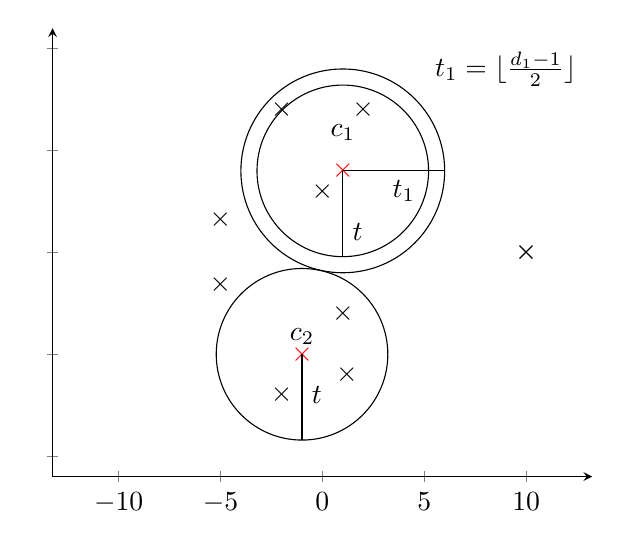
\begin{tikzpicture}
		\begin{axis}[
			axis lines = left,
			xmin=-11, xmax=11, ymin=-11, ymax=11,
			axis equal,
			yticklabels={,,}
			]
			\draw (axis cs: 1, 4) circle [radius=5];
			\draw (axis cs: 1, 4) circle [radius=4.21];
			\draw (axis cs: -1, -5) circle [radius=4.21];
			\node[red] at (1,4){$\times$};
			\node[above] at (1,5){$c_1$};
			\node[red] at (-1,-5){$\times$};
			\node[above] at (-1,-5){$c_2$};
			\node at (2, 7){$\times$};
			\node at (-2, 7){$\times$};
			\node at (0, 3){$\times$};
			\node at (10, 0){$\times$};
			\node at (-5, 1.6){$\times$};
			\node at (1.2, -6){$\times$};
			\node at (-2, -7){$\times$};
			\node at (1, -3){$\times$};
			\node at (10, 0){$\times$};
			\node at (-5, -1.6){$\times$};
			\draw (1,4) -- (6,4);
			\draw (1,4) -- (1,-0.21);
			\node[below] at (4,4){$t_1$};
			\node[right] at (1, 1){$t$};
			\node[right] at (-1, -7){$t$};
			\draw (-1,-5) -- (-1,-9.21);
			\node at (9, 9){$t_1=\lfloor\frac{d_1-1}{2}\rfloor$};
		\end{axis}
	\end{tikzpicture}
\end{center}
Le sequenze che trovo all'interno di questi bound di Hamming sono rappresentabili come $\underline{c_i}+\underline{e}$, in cui ogni vettore $\underline{e}$ rappresenta l'errore introdotto dal canale, e ha una quantità di bit 1 minore o uguale al valore $t_i$ del bound di Hamming.\\
Il numero di sequenze all'interno di ogni bound di Hamming è pari a $$\sum_{r=0}^{t_i}{n\choose r}$$
Prendendo $t$ la distanza minima tra le parole di codice $t=\lfloor\frac{d_{min}-1}{2}\rfloor$, le sequenze che hanno distanza fino a $t$ dalle parole di codice, e che quindi posso correggere, sono $$2^k\sum_{r=0}^t{n\choose r}$$
Il numero di sequenze totali che posso avere è di $2^n$, quindi abbiamo che $$2^k\sum_{r=0}^t{n\choose r}\leq 2^n$$
Sviluppando i calcoli, arrivo ad ottenere che $$\frac{k}{n}\leq1-\frac{1}{n}\log_2\biggl(\sum_{r^0}^t{n\choose r}\biggl)$$ conosciuto come \textbf{bound di Hamming}.\\
Dalla formula ricavata scopro che, aumentando $t$ (ovvero aumentando il numero di errori che voglio correggere), diminuisco il rapporto $\frac{k}{n}$\\

\subsection{Codici lineari a blocco}
Un vettore binario lungo $n$ è una sequenza di $n$ bit.\\
Definisco l'operazione di somma tra due vettori come la somma binaria senza riporto:
$$\underline{x}+\underline{y}=\underline{z}$$
L'insieme degli scalari $\alpha$ è ovviamente $\{0,1\}$:
$$\alpha\underline{x}=\Bigl\{
\begin{array}{c}
	\underline{x}\;\;\;\alpha=1\\
	\underline{0}\;\;\;\alpha=0
\end{array}$$

\subsubsection{Norma}
Definiamo come \textbf{norma di un vettore} (o \textbf{peso di Hamming}) $||\underline{x}||_H$, il numero di $1$ all'interno del vettore.\\
Abbiamo alcune regole per la norma di un vettore:
\begin{enumerate}
	\item $$||\underline{x}||_H\geq0$$
	\item $$||\underline{x}||_H=0\iff\underline{x}=\underline{0}$$
	\item $$||\alpha\cdot\underline{x}||_H=\alpha||\underline{x}||_H$$
	\item $$||\underline{x}+\underline{y}||_H=||\underline{x}||_H+||\underline{y}||_H$$
\end{enumerate}
La distanza indotta dal peso di Hamming è anche la distanza di Hamming: $$||\underline{x}-\underline{y}||_H=d_H(\underline{x},\underline{y})$$
Attenzione che essendo in caso di somme binarie senza riporto, vale la seguente relazione:
$$\underline{x}+\underline{y}=\underline{x}-\underline{y}$$\\
$\mathcal{C}$ è un \textbf{codice lineare a blocco} se $\{\underline{c}_1,...,\underline{c}_{2^k}\}$ è un sottospazio lineare dello spazio binario di dimensione $n$: $\mathcal{C}$ è lineare $\iff\alpha\underline{c}_1+\beta\underline{c}_2\in\mathcal{C}\quad\forall\underline{c}_1,\underline{c}_2$\\

\subsubsection{Peso di Hamming di un codice}
Il \textbf{peso di Hamming di un codice} è il peso di Hamming minimo tra tutte le parole di codice non nulle $$W_H(\mathcal{C})=min||\underline{c}||_H\qquad\underline{c}\in\mathcal{C}\backslash\{\underline{0}\}$$\\
In un codice lineare a blocco, il peso di Hamming del codice, coincide con la distanza minima del codice $$W_H(\mathcal{C})=min\big(d_H(\underline{\gamma}_1, \underline{\gamma}_2)\big)$$
In quanto il codice è lineare, la distanza di Hamming tra due parole di codice, ovvero la differenza tra i due vettori, è il peso di Hamming di una parola di codice: $d_H(\underline{\gamma}_1,\underline{\gamma}_2)=||\underline{c}||_H,\quad c\in\mathcal{C}$, quindi abbiamo che $$W_H(\mathcal{C})=min\big(d_H(\underline{\gamma}_1,\underline{\gamma}_2)\big)=min||\underline{c}||_H,\qquad c\in\mathcal{C}\backslash\{0\}$$
\subsubsection{Matrice generatrice di un codice lineare}
Una matrice $\underline{G}$ è matrice generatrice del codice $\mathcal{C}$ se la generica parola di codice può essere scritta come 
\begin{gather*}
	\underline{c}=\underline{G}\;\underline{b}\\\\
	\underline{c}=
	\left (\;
	\begin{array}{c}
		c_1\\
		.\\
		c_n\\
	\end{array}
	\;\right )\qquad
	\underline{b}=
	\left(\;
	\begin{array}{c}
		b_1\\
		.\\
		b_k
	\end{array}
	\;\right)\\\\
	\underline{G}=
	\left(\;
	\begin{array}{ccc}
		G_{1,1}&.&G_{1,k}\\
		.&.&.\\
		G_{n,1}&.&G_{n,k}
	\end{array}
	\;\right
	)
\end{gather*}
per ogni vettore $\underline{b}$\\
Le colonne di $\underline{G}$ sono \textbf{linearmente indipendenti}, altrimenti non potrei avere $2^k$ diverse parole di codice.\\
Cambiare l'ordine delle righe di $\underline{G}$ cambia l'ordine dei bit in ogni parola di codice, ottenendo un codice diverso: usando questo codice, dato che il peso di Hamming non viene modificato, la distanza tra le parole di codice non cambia, mantenendo le stesse prestazioni e probabilità d'errore del codice originale.\\
Da una qualsiasi matrice generatrice posso sempre ottenere una matrice generatrice $\underline{G}'$ di un codice equivalente in forma sistematica utilizzando combinazioni lineari delle colonne o permutazioni delle righe.\newpage
Con matrice $\underline{G}$ sistematica:
$$\underline{G}=
\left(\;\begin{array}{c}\underline{I}\\\\
	\hline\\
	\underline{A}
\end{array}\;\right)\qquad\underline{I}[k\times k],\;\underline{A}[(n-k)\times k]$$
generando le parole di codice
$$\underline{c}=
\left(\;\begin{array}{c}\underline{b}\\\\
	\hline\\
	\underline{A}\;\underline{b}
\end{array}\;\right)$$

\subsubsection{Bound di Singleton}
Per codici lineari a blocco $(n,k)$, la distanza minima del codice è limitata superiormente $$d_{min}\leq n-k+1$$
in quanto una matrice $\underline{G}$ in forma sistematica avrà come massimo $1+n-k$ uni per colonna.
$$\underline{G}=\left(\;\begin{array}{c}\underline{I}\\\\\hline\\\underline{A}\end{array}\;\right)\qquad\underline{I}[k\times k],\;\underline{A}[(n-k)\times k]$$
Come conseguenza di questa conclusione c'è il fatto che non possiamo quindi distanziare troppo le parole di codice tra loro, impedendoci di abbassare troppo la probabilità d'errore.\\

\subsection{Decodifica dei codici lineari}
Una matrice di controllo di parità di un codice lineare $\mathcal{C}$ soddisfa
$$\underline{H}\underline{\gamma}=\underline{0}\iff\underline{\gamma}\in\mathcal{C}$$ tecnica utile per determinare se un vettore $\underline{\gamma}$ è una parola del codice.\\
$\underline{H}$ è matrice di controllo di parità di un codice con matrice generatrice $\underline{G}$ se e solo se 
$$\underline{H}\,\underline{G}=\underline{0}\quad e \quad rango(\underline{H})=n-k$$
TODO lezione 26










\newpage
\section{Teoria dell'informazione}
Facciamo riferimento a uno spazio degli eventi $\Omega$, mentre sottoinsiemi di $\Omega$ rappresentano eventi distinti $A\subseteq\Omega$.\\
Sullo spazio degli eventi, definiamo la probabilità $P$

\subsection{Assiomi dell'informazione}
L'informazione è una funzione dell'evento $A$ ($i(A)$ importanza/quantità dell'informazione) in cui vale:
\begin{enumerate}
	\item $i(A)\geq0,\qquad\forall A$\\
	L'informazione deve esserci per esistere.
	\item $P(A)\leq P(B),\qquad i(A)\geq i(B)$\\
	Se un'informazione è \textbf{meno probabile}, allora sarà \textbf{più importante}.
	\item $i(\Omega)=0$\\
	Siccome $\Omega$ è lo spazio degli eventi, la probabilità che accada $\Omega$ è 1, quindi \textbf{non è importante dato che accade sicuramente}.
	\item Se $A$ e $B$ sono eventi indipendenti allora $i(\{A\land B\})=i(A)+i(B)$ (ricordiamo che $P(a\land B)=P(A)P(B)$)
\end{enumerate}
Andando ad analizzare matematicamente l'informazione relativa ad un evento proviamo a spiegarla tramite la relazione
$$i(A)=\pm\log_{\_}(P(A))$$
Andiamo a verificare se gli assiomi valgono:
\begin{enumerate}
	\item Siccome la probabilità è compresa tra 0 e 1, il logaritmo ha risultati negativi: dobbiamo usare il meno
	\item $-\log$ è una funzione decrescente, quindi all'aumentare della probabilità, diminuisce l'informazione
	\item $P(\Omega)=1\rightarrow\log(1)=0$
	\item $i(A+B)=-\log(P(A\land B))=-(\log(P(A)P(B)))=-(\log(P(A))+\log(P(B))=i(A)+i(B)$
\end{enumerate}
La relazione trovata quindi diventa:
$$i(A)=-\log_b(P(A)),\qquad b>1$$
Usando la base 2, l'informazione sarà \textbf{rappresentabile in bit}.\\
Usando la base $e$, l'unità di misura diventa il \textbf{Neper}.\\\\

\subsection{Funzione informazione di una variabile aleatoria discreta}
Sia $X$ una variabile aleatoria discreta con densità di probabilità $p_x(x)$:
$$x\in A_x=\{a_1,...,a_n\}$$
$$p_x(a)=P(X=a),\;a\in A_x$$
Definiamo la \textbf{funzione informazione} come
$$i_x(a)=i(\{x=a\})=-\log_2(p_x(a))$$

\subsubsection{Informazione di eventi di X}
$$x\in A_x=\{a_1,...,a_n\}$$
Dato un insieme $B\subseteq A_x$,
$$i(B)=l\log_2(P(B))=-\log_2(\sum_{a\in B}p_x(a))$$
Noto quindi che la funzione informazione non mi serve per calcolare l'informazione di un evento specifico, devo per forza passare per la densità di probabilità.\\

\subsection{Entropia di una variabile aleatoria}
Data una v.a. discreta $X$, l'entropia di $X$ è definita come l'\textbf{informazione media} di $X$:
$$H(x)=E[i_x(x)]=\sum_{a\in A_x}p_x(a)\log_2(\frac{1}{p_x(a)})$$
L'entropia mi rappresenta l'informazione media portata dall'informazione, quindi la novità portata dalla realizzazione di un determinato evento.\\
Un altro modo per vedere l'entropia è che l'entropia mi rappresenta l'incertezza complessiva sulla variabile aleatoria.

\subsubsection{Proprietà dell'entropia}
\begin{enumerate}
	\item $H(X)\geq0$
	\item $H(X)=0$ solo se $X$ è deterministica
\end{enumerate}

\subsection{Funzioni concave e diseguaglianza di Jensen}
Una funzione $f(x)$ è strettamente concava, dati $k_1,...,k_N\geq0$, tali che $\sum_{n=1}^Nk_n=1$ e dati $a_1,...,a_N$ distinti, se vale che
$$\sum_{n=1}^Nk_nf(a_n)<f(\sum_{n=1}^N(k_na_n))$$

\subsubsection{Disequazione di Jensen}
Sia $X$ v.a. e $f(x)$ una funzione strettamente concava:
$$E[f(x)]=\sum_{a\in A_x}p_x(a)f(a)$$
$$E[f(x)]<f\biggl(\sum_{a\in A_x}p_x(a)a\biggl)=f(E[x])$$
Si ha quindi che
$$E[f(x)]<f(E[x])$$

\subsection{Limite superiore dell'entropia di una v.a. discreta}
Sia $X$ una v.a. discreta $X\in A_x$; indichiamo con M la cardinalità dell'alfabeto $M=|A_x|$.\\
Il \textbf{limite superiore dell'entropia} di $X$ è
$$H(x)\leq \log_2(M)$$
inoltre $H(x)=\log_2(M)\iff X$ è uniforme in $A_x$.\\\\
Dim:
$$H(x)=E[-\log_2(p_x(x))]$$
Ricordando che $\log_2(a)$ è strettamente concava, sfruttiamo la disequazione di Tensen:
$$H(x)=E[\log_2(\frac{1}{p_x(x)})]<\log_2\biggl(E[\frac{1}{p_x(x)}]\biggl)=\log_2\biggl(\sum_{a\in A_x}\frac{p_x(a)}{p_x(a)}\biggl)=\log_2(M)$$
La disequazione vale solo se i valori di $p_x(x)$ sono distinti tra loro.\\
Se $X$ è uniforme nell'alfabeto ($p_x(a)=\frac{1}{M}).$
$$H(X)=E[\log_2(\frac{1}{p_x(x)})]=\sum_{a\in A_x}\frac{1}{M}\log_2(\frac{1}{\frac{1}{M}})=\frac{1}{M}\sum_{m=1}^M\log_2(M)=\log_2(M)$$

\subsection{Vettori aleatori}
Un vettore aleatorio di lunghezza N $\underline{X}=[X_1,...,X_N],\; n\in[1,N]$ con $X_n$ variabile aleatoria discreta con alfabeto $A_n$, $\underline{X_n}\in A_1\times ...\times A_N=A$.\\
La densità di probabilità del vettore aleatorio $p_{\underline{x}}(\underline{a})=P(\underline{X}=\underline{a}),\quad \underline{a}\in A$

\subsection{Funzione informazione per un vettore aleatorio}
Definito quindi il vettore aleatorio, abbiamo che la funzione informazione, per un vettore aleatorio, è:
$$i_{\underline{x}}(\underline{a})=\log_2\Big(\frac{1}{p_{\underline{x}}(\underline{a})}\Big)$$

\subsection{Entropia di una variabile aleatoria}
L'entropia di un vettore aleatorio, come per una variabile aleatoria discreta, è $$H(X)=E\big[i_{x}(X)]\big]=\sum_{{a}\in A}p_{{x}}({a})\log_2\big(\frac{1}{p_{{x}}({a})}\big)$$

\subsection{Entropia di più variabili aleatorie}
Consideriamo due v.a. ${X}$ ${Y}$.\\
\begin{enumerate}
	\item Se ${X}$ e ${Y}$ sono \textbf{indipendenti}: $$H({X},{Y})=E\big[i_{x,y}({X},{Y})\big]=E\big[i_x(a)+i_y(b)\big]=H({X})+H({Y})$$
	\item Se ${X}$ e ${Y}$ \textbf{non sono indipendenti}: $$H({X},{Y})<H({X})+H({Y})$$
	\item Se $f({X})={Y}$ è \textbf{funzione deterministica}: $$H({X}, {Y})=H({X})$$
	La cosa tuttavia non ci sorprende in quanto l'entropia esprime l'incertezza sulla coppia, e essendo ${Y}$ funzione deterministica di ${X}$, l'incertezza della coppia è quella di ${X}$.\\
	Attenzione che non vale in generale il contrario, ovvero $$H({X},{Y})\neq H({Y})$$
	\item Se ${Y}$ \textbf{non è funzione deterministica} di ${X}$: $$H({X},{Y})>H({X})$$	
	\item Se $f({X})={Y}$ è \textbf{funzione iniettiva}, la densità di probabilità di ${X}$ è la stessa di ${Y}$ a meno di una modifica dell'alfabeto: $$H({X})=H({Y})=H({X},{Y})$$
\end{enumerate}
Volendo raccogliere tutte le diseguaglianze ricavate, abbiamo la seguente catena:
$$0\leq max\{H({X},{Y})\}\leq H({X},{Y})\leq H({X}+{Y})$$
Vale sempre che $H({X},{Y})=H({Y},{X})$.\\

\subsubsection{Variabili aleatorie condizionate}
Data la v.a. $X$ condizionata alla variabile aleatoria $Y$ con densità di probabilità condizionata $p_{x|y}(a|b)=P(X=a|Y=b)$, definiamo la funzione informazione condizionata come
$$i_{x|y}(a|b)=\log_2\big(\frac{1}{p_{x|y}(a|b)}\big)$$
\textbf{Entropia condizionata ad un certo valore di $y$}: $$H(X|Y=b)=\sum_{a\in A_x}p_{x|y}(a|b)\log_2\big(\frac{1}{p_{x|y}(a|b)}\big)$$
In generale
$$H(X|Y)=E_y\big[H(X|Y=y)\big]=\sum_bp_y(b)H(X|Y=b)$$
Sviluppando i calcoli nella sommatoria, otteniamo un tipo di entropia diversa dal solito:
$$H(X|Y)=\sum_{a,b}p_{x,y}(a,b)\log_2\big(\frac{1}{p_{x|y}(a|b)}\big)$$
Il nostro scopo è quello di scrivere l'entropia condizionata in funzione dell'entropia congiunta... sviluppando i calcoli nella sommatoria, si ottiene:
$$H(X,Y)=H(X|Y)+H(Y)$$
Questa conclusione si poteva ricavare anche dalla relazione tra probabilità congiunta e probabilità condizionata, in quanto l'entropia è una funzione logaritmica e trasforma i prodotti in somme.

\subsection{Informazione mutua tra due variabili aleatorie}
$$I(X;Y)=I(Y;X)=H(X)+H(Y)-H(X,Y)$$
Dalla relazione trovata tra entropia condizionata e congiunta possiamo semplificare la formula dell'informazione mutua:
$$I(X;Y)=H(X)-H(X|Y)=H(Y)-H(Y|X)$$
A livello logico, sto togliendo dall'informazione che mi porta $X$, l'informazione su $X$ che già sapevo data l'informazione $Y$.\\
$H(X|Y)$ misura \textbf{quanto non so di x dopo che ho visto y}.\\
$I(X;Y)$ misura \textbf{quando so di x dopo aver visto y}.\\

\subsubsection{Valori assunti dalla mutua informazione}
$$I()X;Y)=H(X)+H(Y)-H(X,Y)\geq0$$
In quanto sappiamo che l'entropia congiunta vale meno della somma delle entropie di $X$ e $Y$ (è impossibile avere un'informazione nulla, l'informazione o esiste (>0) o non esiste (=0)).\\
$$I(X;Y)=H(X)-H(X|Y)\leq min\{H(X),H(Y)\}$$
Si ha quindi che $$0\leq I(X;Y)\leq min\{H(X),H(Y)\}$$

\subsection{Entropia per simbolo di un vettore aleatorio}
Dato un vettore aleatorio $\underline{X}=[X_1,...,X_N]$, l'entropia per simbolo del vettore è $$H_s(\underline{X})=\frac{1}{N}H(\underline{X})$$
Se gli elementi del vettore aleatorio $\underline{X}$ sono \textbf{identicamente distribuiti} ($p_{X_i}(a)=p_{X_j}(a),\;\forall i$), abbiamo che l'entropia per simbolo coincide con l'entropia del vettore aleatorio $$H_s(\underline{X})=\frac{1}{N}H(\underline{X})=H(X)$$
dato che, in quanto identicamente distribuiti, $H(\underline{X})=NH(X)$.

\subsection{Informazione mutua per simbolo}
$$I_s(\underline{X};\underline{Y})=H_s(\underline{X})+H_s(\underline{Y})-H_s(\underline{X},\underline{Y})$$

\subsection{Sorgente di simboli}
Se abbiamo una sorgente che in un tempo infinito genera un numero infinito di simboli, abbiamo un vettore aleatorio $\underline{X}=[...,X_{-1},X_0,X_1,...]$ di dimensione infinita.\\
L'entropia di solito è infinita in tutto il vettore, se questo è infinitamente lungo; l'entropia per simbolo invece sarà $$H_s(\underline{X})=\lim_{N\to\infty}\frac{1}{2N+1}H(\underline{X}=[X_{-N},...,X_N])$$

\subsection{Tasso di informazione di un messaggio}
Una sorgente genera simboli $X_i$ ad intervalli di tempo $T=$periodo di simbolo.\\
Il tasso di informazione (information rate) del messaggio generato dalla sorgente è $$R(\underline{X})=\frac{H_s(\underline{X})}{T}\qquad[bit/s]$$

\subsection{Tasso nominale del messaggio}
Il tasso nominale del messaggio con $X_i\in A$ con $A$ di cardinalità $M$ è $$\frac{\log_2(M)}{T}$$

Il tasso di informazione di un messaggio mi dice \textbf{quanta informazione viene generata dalla sorgente al secondo}, mentre il tasso nominale del messaggio mi dice semplicemente \textbf{quanti bit vengono trasmessi} (non per forza contenenti informazione $i=0$).\\
Ovviamente il tasso nominale del messaggio fungerà come limite superiore del tasso di informazione di un messaggio, in quanto non può essere trasmessa più informazione di quanti bit vengono trasmessi
$$R(\underline{X})\leq \frac{\log_2(M)}{T}$$








\newpage
\section{Codifica di canale}
Indichiamo con $T_c$ il \textbf{tempo di simbolo del canale}.

\subsection{Canale numerico M-ario senza memoria}
Essendo un canale numerico, $x_n, y_n\in\{a_1,...,a_M\}$, ed essendo senza memoria, $y_n$ dipende solo da $x_n$ e non dai simboli trasmessi precedentemente.\\

\subsubsection{Descrizione del canale attraverso una matrice di probabilità di transizione}
$$P(y_n=a|x_n=b)=\left(\;\begin{array}{ccc}
	P(1,1)&\cdot&P(1,M)\\\\
	\cdot&\cdot&\cdot\\\\
	P(M,1)&\cdot&P(M,M)
\end{array}\;\right)$$

Sommando i valori della colonna $i$ della matrice, a patto che ogni simbolo sia trasmesso con la stessa probabilità, ottengo $P_{y_n}(i)$; sommando le colonne della matrice, invece, ottengo 1.\\

\subsubsection{Tasso di informazione del canale}
Definiamo $\mathcal{G}$ un canale numerico M-ario senza memoria, con probabilità di transizione $P(y_n|x_n)$.\\
Il tasso di informazione di $\mathcal{G}$ è (per una certa statistica della sorgente) 
$$R(\mathcal{G})=\frac{1}{T_c}I_s(\underline{x};\underline{y})=\frac{1}{T_c}\big[H_s(\underline{x})+H_s(\underline{y})-H_s(\underline{x},\underline{y})\big]\qquad[bit/s]$$
Se $x_n$ e $y_n$ sono \textbf{indipendenti} ((in $n$) e \textbf{identicamente distribuiti}:
$$R(\mathcal{G})=\frac{1}{T_c}I_s(x_n;y_n)$$
Per esempio, nel caso in cui abbiamo $y_n=x_n$, la matrice di probabilità di transizione è uguale alla matrice identità; il tasso di informazione del canale vale $R(\mathcal{G})=\frac{1}{T_c}H(x_n)$.\\
In generale, per un canale qualsiasi, poichè $I_s(\underline{x};\underline{y})\leq H_s(\underline{x})$, avremo che $$R(\mathcal{G})=\frac{I_s(\underline{x};\underline{y})}{T_c}\leq\frac{H_s(\underline{x})}{T_c}$$

\subsubsection{Capacità di un canale numerico M-ario senza memoria}
La capacità del canale è il \textbf{massimo tasso di informazione del canale} tra tutti quelli ottenuti, usando tutte le possibili distribuzioni della sorgente $$C=max\big(R(\mathcal{G})\big)$$
Nell'esempio di prima ($y_n=x_n$), la capacità è $$C=\frac{\log_2(M)}{T_c}$$ (ottenuta con $x_n$ a valori equiprobabili nell'alfabeto M-ario)

\subsection{Teorema di Shannon per la codifica di canale}
Consideriamo un canale M-ario numerico senza memoria con periodo di simbolo $T_c$ e capacità $C$.\\
Sia $\{b_{\mathcal{C}}\}$ una sorgente con tasso di informazione del messaggio nominale $R$.\\
Se $R<C$, allora per ogni $\delta>0$ e per ogni $n$ sufficientemente grande, esistono:
\begin{enumerate}
	\item Un \textbf{codice di canale} con parole (con alfabeto M-ario) lunghe $n$ e con un numero di parole $\lceil2^{nRT_c}\rceil$
	\item Un \textbf{decodificatore per il codice} tali che la probabilità di errore sulla parola di codice è minore di $\delta$
\end{enumerate}
Il numero di parole di codice dal teorema è $$2^{nRT_c}=2^k$$ per un codice a blocco (n,k); si ha quindi che $$\frac{k}{n}=RT_c<CT_c$$

\subsubsection{Converse}
Per un canale M-ario numerico senza memoria e con capacità $C$, esiste $\delta>0$ tale che per un qualsiasi codice e strategia di decodifica, se $R\geq C$ (con $R$ tasso di informazione nominale della sorgente), la probabilità di errore sulla parola di codice è sempre $\geq\delta$.\\

\subsection{Canale analogico AWGN}

\subsubsection{Capacità di un canale analogico AWGN}
$$r(t)=s_{T_X}(t)+w(t)$$
Con $s_{T_X}(t)$ segnale analogico e $w(t)$ rumore AWGN (V.A. Normale con media nulla).\\
La capacità di questo tipo di canale è $$C=\frac{1}{T}\log_2\big(1+\frac{\sigma_{s_{Tx}}^2}{\sigma_w^2}\big)$$
con $\sigma_{s_{Tx}}^2=E\big[s_{T_X}^2(t)\big]$ e $\sigma_w^2$ la varianza del rumore.\\
La densità di probabilità dell'ingresso che massimizza la mutua informazione (che raggiunge la capacità calcolata) è Gaussiana a media nulla (per una potenza fissata).\\

\subsection{Canale binario simmetrico senza memoria}
$$P(\hat{b_l}=1|b_l=0)=P(\hat{b_l}=0|b_l=1)=P_{bit}$$ (simmetrico)\\
$$C=max\big(\frac{I(b_l;\hat{b_l})}{T_b}\big)$$
L'informazione mutua abbiamo che vale $$I(b_l;\hat{b_l}) = H(\hat{b_l})-H(\hat{b_l}|b_l)$$
facendo i calcoli otteniamo che $$C=\frac{1}{T_C}\big\{1-\big[P_{bit}\log_2(\frac{1}{P_{bit}})+(1-P_{bit})\log_2(\frac{1}{1-P_{bit}})\big]\}$$

\subsection{Canale binario senza memoria con cancellazione}
Si tratta di un canale che ha \textbf{in ingresso due possibili simboli} $(0,1)$ ma \textbf{con uscita tre possibili valori} $(0,1,e)$.\\
Posso avere una possibilità che avendo trasmesso $1$ io riceva $e$ (lo stesso vale per lo $0$).
$$\begin{array}{c}
	P(y=e|x=0)=P(y=e|x=1)=\alpha \\\\
	P(y=0|x=0)=P(y=1|x=1)=1-\alpha \\\\
	P(y=1|x=0)=P(y=0|x=1)=0
\end{array}$$
Posso trovare un canale di questo tipo ad esempio se considero una modulazione di canale binaria e sono troppo incerto al ricevitore (se non so cosa ho trasmesso, non mi prendo rischi e non decodifico il messaggio).
\begin{center}
	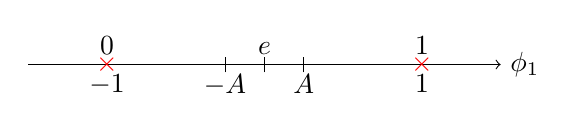
\begin{tikzpicture}
		\draw[->] (-3,0) -- (3,0) node[right]{$\phi_1$};
		\node[red] at (-2,0){$\times$};
		\node[above] at (-2,0){$0$};
		\node[below] at (-2,0){$-1$};
		\node[above] at (0,0) {$e$};
		\draw[color=black] (0,-0.1) -- (0,0.1);
		\node[below] at (0.5,0) {$A$};
		\draw[color=black] (0.5,-0.1) -- (0.5,0.1);
		\node[below] at (-0.5,0) {$-A$};
		\draw[color=black] (-0.5,-0.1) -- (-0.5,0.1);
		\node[red] at (2,0){$\times$};
		\node[above] at (2,0){$1$};
		\node[below] at (2,0){$1$};
	\end{tikzpicture}
\end{center}
$$\alpha=P\big(w\in[-(1+A);-(1-A)]\big)$$
Essendo però in un canale con rumore gaussiano, non è mai nulla la probabilità che venga ricevuto 0 dato che è stato trasmesso 1, quindi dovremmo (a scopo matematico) introdurre un'altra probabilità: $$\beta = P\big(y=1|x=0\big)=P\big(w>(1+A)\big)\simeq 0$$
Fissando $q=P(x=0)$ abbiamo che:
$$\begin{array}{c}
	P_y(0)=q(1-\alpha)\\\\
	P_y(1)=(1-q)(1-\alpha)\\\\
	P_y(e)=\alpha
\end{array}$$
Calcoliamo quindi ora la capacità del canale:
$$C=\frac{1}{T}max\big(I(x;y)\big)=\frac{1-\alpha}{T}$$













\newpage
\section{Codifica di Sorgente}
L'operazione di codifica di sorgente, codifica il flusso di informazione e lo converte in un'altra sequenza di simboli.\\
Lo scopo del processo è \textbf{comprimere il messaggio}, in modo da trasmettere il minor numero di $bit/s$.\\
Dopo la codifica di sorgente, avvengono la codifica di canale, la modulazione, la demodulazione, la decodifica di canale e in fine la decodifica di sorgente.\\
Ci sono \textbf{due tipi di codifiche di sorgente}:
\begin{enumerate}
	\item \textbf{Codifica di sorgente senza perdite (LOSSLESS)}: Il messaggio all'uscita del decodificatore coincide con quello all'ingresso del codificatore.
	\item \textbf{Codifica di sorgente con perdite (LOSSY)}: Il messaggio all'uscita del decodificatore è simile ma non coincide con quello all'ingresso del codificatore.
\end{enumerate}

\subsection{Codifica di sorgente senza perdite}
La sorgente trasmette da un dizionario $\mathcal{D}_x$ delle parole $\underline{x}$ con una densità di probabilità $p_x$.\\
In generale, all'uscita dal codificatore di sorgente, le parole saranno più corte; le parole in uscita allora faranno parte di un alfabeto $\mathcal{D}_y$ delle parole $\underline{y}$ con lettere prese da un alfabeto con cardinalità $M_y$.\\
Le parole $\underline{y}$ hanno una \textbf{lunghezza variabile} (in generale), in quanto ho una miglior dinamicità per la creazione delle parole in uscita e non ho le mani legate per come creare il codificatore (possono esserci \textbf{parole più corte che corrispondono a parole lunghe più probabili}).\\
Quello che conta è la lunghezza media media delle parole $\underline{y}$: $$L_y=E\big[L(\underline{y})\big]=\sum L(\underline{y})p_{\underline{x}}(\underline{x}(\underline{y}))$$
con $\underline{x}(\underline{y})$ si intende la parola $\underline{x}$ associata alla parola codificata $\underline{y}$ e con $L(\underline{y})$ la funzione che mi determina la lunghezza della parola $\underline{y}$.\\\\
Il codificatore di canale, tuttavia, vuole blocchi di lunghezza fissa, mentre il codificatore di sorgente, cercando di comprimere, trasmette \textbf{blocchi con lunghezza variabile}.\\
Per risolvere a questo problema, prendo le parole trasmesse dal codificatore di sorgente e le unisco in un unica grande parola; il codificatore di canale poi suddividerà l'unione delle parole in parole della lunghezza necessaria. Se poi non ci saranno errori nel canale sarà possibile ricostruire la sequenza di parole iniziale.\\

\subsubsection{Codici a prefisso}
Per riuscire a suddividere le parole che erano state unificate dal codificatore di canale, utilizzo i \textbf{codici a prefisso}: un codice di sorgente a prefisso \textbf{non ha nessuna parola di codice che è prefisso di un'altra}.\\
Ad esempio il dizionario $\mathcal{D}_y=\{0,10,111\}$ è un codice a prefisso in quanto ogni parola di codice non è utilizzabile come prefisso di un'altra parola.\\

\subsection{Teorema di Kraft Mc-Millan}
\begin{enumerate}
	\item Per ogni codificatore di sorgente senza perdite, deve valere $$\sum_{\underline{b}\in\mathcal{D}_y}\frac{1}{M_y^{L_{\underline{y}}(\underline{b})}}\leq 1$$ dove $M_y$ è la cardinalità dell'alfabeto di $\underline{y}$ e $L_y(\underline{b})$ è la lunghezza (in simboli) della parola $\underline{b}$
	\item Per una sorgente con dizionario di cardinalità $N$ (con $N$ parole da codificare), se $l_1,...,l_N$ sono interi che verificano $$\sum_{i=1}^N\frac{1}{M_y^{l_i}}\leq 1$$ con $M_y$ intero, allora esiste un codice a prefisso con alfabeto di cardinalità $M_y$ e parole di codice di lunghezza $L_i$
\end{enumerate}

\subsection{Teorema di Shannon per la codifica di sorgente}
\begin{enumerate}
	\item Per ogni codice di sorgente con alfabeto di cardinalità $M_y$, la lunghezza media delle parole soddisfa $$L_y\geq \frac{H(\underline{X})}{\log_2(M_y)}$$
	\item Esiste un codice a prefisso con alfabeto di cardinalità $M_y$ e lunghezza media delle parole di codice $$L_y<\frac{H(\underline{x})}{\log_2(M_y)}+1$$
\end{enumerate}
Il teorema di Shannon \textbf{lega la lunghezza media delle parole di codice all'entropia della sorgente}.\\
Unendo le cose, otteniamo che $$\frac{H(\underline{x})}{\log_2(M_y)}\leq L_y<\frac{H(\underline{x})}{\log_2(M_y)}+1$$
sempre se faccio le cose per bene (si tratta di una garanzia di esistenza, non garantisce che ogni codifica di sorgente avrà questo risultato).\\
Abbiamo quindi che la lunghezza delle parole di codice hanno lunghezza $$l_i=\lceil\log_{\frac{1}{M_y}}(p_x(a_i))\rceil\qquad\forall a_i\in\mathcal{D}_x$$
Il codice con queste lunghezze si chiama \textbf{Codice di Shannon-Fano}.\\
Il codice di Shannon-Fano è ottimo (raggiunge la lunghezza media minima tra tutti i codici per una data sorgente) se $p_x(a_i)$ sono \textbf{potenze intere} di $\frac{1}{M_y}$ in modo che il logaritmo dia un numero intero.\\
$$L_y=E\big[\log_{\frac{1}{M_y}}(p_x(a_i))\big]=\frac{H(\underline{x})}{\log_2(M_y)}$$

\subsection{Codifica di sorgente ottima}
Per un codice a prefisso ottimo, parole a più bassa probabilità hanno lunghezza maggiore $$p_x(a_1)\geq p_x(a_2)\rightarrow L(b_1)\leq L(b_2)$$
\subsubsection{}
Nel dizionario di un codice a prefisso ottimo, ci sono almeno due parole di codice $\underline{b}'$ e $\underline{b}''$ che hanno lunghezza massima e differiscono solo nell'ultimo simbolo.\\

\subsection{Procedura di Huffman}
Fornisce un codice di sorgente ottimo data la densità di probabilità del dizionario $\mathcal{D}_x$ da codificare.
\begin{enumerate}
	\item Ordiniamo le parole di $\mathcal{D}_x$ con probabilità decrescente $$p_x(a_1')\geq...\geq p_x(a_{N-1}')\geq p_x(a_N')$$
	\item Assegnamo le parole pià lunghe a $a_{N-1}'$ e $a_N'$ e le costruiamo uguali tranne l'ultimo bit
	\item Costruisco un nuovo codice sul dizionario con densità di probabilità\\ $p(a_1'),\,...,\,p(a_{N-1}'),\,p(a_N')$
\end{enumerate}

\subsection{Codifica aritmetica}

\subsubsection{Codice di Elias}
Data una densità di probabilità delle parole di ingresso $\mathcal{D}_x)\{a_1,..,1_N\}$, $p_x(a_1),\,...,\,p_x(a_N)$; supponiamo che le parole abbiano un ordine (es lessicografico)\\
TODO: Recupero ultima lezione da Bisca

\end{document}
